\section{Apache Hadoop}\label{sec:hadoop}

Apache Hadoop ist ein Open-Source-Software-Projekt, mit dessen Hilfe ermöglicht wird, Programme zur Datenverarbeitung mit großen Ressourcenbedarf auf verteilten System auszuführen. Hadoop wird von der \emph{Apache Foundation} entwickelt und bietet verschiedene Komponenten an, welche vollständig skalierbar sind, von einer einfachen Installation auf einem PC bis hin zu einer Installation über mehrere Server in einem Serverzentrum. Hadoop besteht hauptsächlich aus folgenden Kernmodulen \cite{HadoopHomePage}:

\begin{description}
	\item[Hadoop Common] Gemeinsam genutzte Kernkomponenten
	\item[Hadoop YARN] Framework zur Verteilung und Ausführung von Tasks und das dazugehörige Ressourcen-Management
	\item[Hadoop Distributed File System] Kurz HDFS, Verteiltes Dateisystem
	\item[Hadoop MapReduce] YARN-Basiertes System zum Verarbeiten von großen Datenmengen
\end{description}

Hadoop ermöglicht es dadurch, sehr einfach mit Tasks umzugehen, welche große Datenmengen verarbeiten. Da es für Hadoop nicht relevant ist, auf wie vielen Servern es läuft, kann es beliebig skaliert werden, wodurch entsprechend viele Ressourcen zur Bearbeitung und Speicherung von großen Datenmengen zur Verfügung stehen können.

\begin{figure}
	\centering
	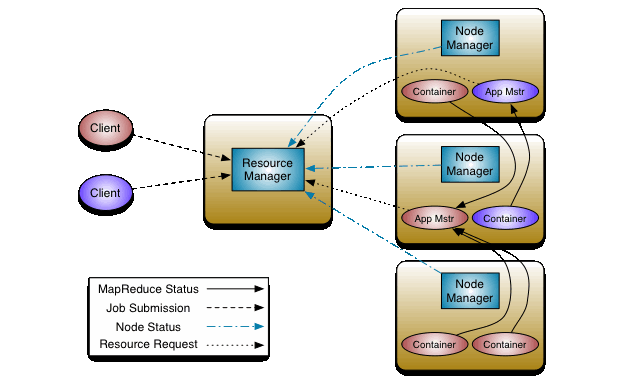
\includegraphics[width=\columnwidth]{./images/yarn_architecture.png}
	\caption[Architektur von YARN]{Architektur von YARN \cite{HadoopYarnArch271}}
	\label{fig:yarnarch}
\end{figure}

Die Kernidee der Architektur von \textbf{YARN} ist die Trennung vom Ressourcenmanagement und Scheduling. Dazu besitzt der Master bzw. \texttt{Controller} den \ac{RM}, welcher für das gesamte System zuständig ist und die Anwendungen im System überwacht. Er besteht aus zwei Kernkomponenten, dem \ac{AM} und dem \emph{Scheduler}. Der \ac{AM} ist für die Annahme und Ausführung von einzelnen Anwendungen zuständig, denen der Scheduler die dafür notwendigen Ressourcen zuteilt und überwacht. Für jeden Slave-\emph{Node} im Hadoop-System gibt es dazu einen \ac{NM}, welcher die lokalen Ressourcen des Nodes überwacht und dem \ac{RM} mitteilt. Jede Anwendung besitzt jeweils einen eigenen \ac{AppMstr}, welcher für das Monitoring und die Kommunikation mit dem \ac{RM} und \ac{NM} zuständig ist und die dazu notwendigen Informationen bereit stellt. Jede YARN-Anwendung bzw. Job besteht aus einem oder mehreren \emph{Containern}, in denen die einzelnen Tasks der Anwendung auf einem beliebigen Node ausgeführt werden \cite{HadoopYarnArch271}.

\begin{figure}
    \centering
    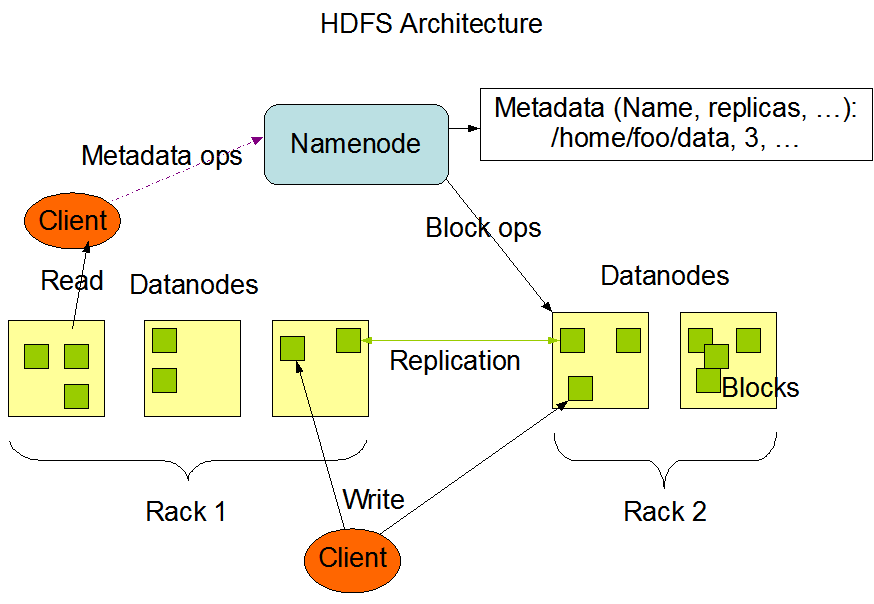
\includegraphics[width=.8\columnwidth]{./images/hdfsarchitecture.png}
    \caption[Architektur des HDFS]{Architektur des HDFS \cite{HadoopHdfsDesc271}}
    \label{fig:hdfsarch}
\end{figure}

Das \textbf{HDFS} basiert auf der gleichen Architektur wie YARN und besitzt ebenfalls einen Master und mehrere Slaves, welches in der Regel die gleichen Nodes sind wie bei YARN sind. Der \emph{NameNode} ist als Master für die Verwaltung des Dateisystems zuständig und reguliert den Zugriff auf die darauf gespeicherten Daten. Die Daten selbst werden in mehrere Blöcke aufgeteilt auf den \emph{DataNodes} gespeichert. Um den Zugriff auf die Daten im Falle eines Node-Ausfalls zu gewährleisten, wird jeder Block auf anderen Nodes repliziert. Dateioperationen (wie Öffnen oder Schließen) werden direkt auf den DataNodes ausgeführt, sie sind darüber hinaus auch dafür verantwortlich, dass Clients die Daten lesen oder beschreiben können \cite{HadoopHdfsDesc271}.

\textbf{MapReduce} bietet analog zu YARN die Möglichkeit, Anwendungen mit einem großen Ressourcenbedarf, welche große Datenmengen verarbeiten, auf einem gesamten Cluster auszuführen. Dazu werden bei einem MapReduce-Job die Eingabedaten aufgeteilt, anschließend von den sog. \emph{Map Tasks} verarbeitet und deren Ausgaben von den sog. \emph{Reduce Tasks} geordnet. Für die Ein- und Ausgabe der Daten wird in der Regel das HDFS, für die Ausführung der einzelnen Tasks YARN genutzt \cite{HadoopMapRedTutorial271}. MapReduce kann man auch als Vorgänger von YARN ansehen, da YARN auch als \emph{MapReduce Next Gen} oder \emph{MRv2} bezeichnet wird und erst in einer späteren Version von Hadoop implementiert wurde \cite{HadoopYarnOverview271}.

%Hier soll Hadoop in einer modifizierten Variante zum Einsatz kommen. In \cite{zhang2016} haben Zhang et. al. eine Verbesserung des Scheduler des ResourceManagers vorgestellt, welche genutzt werden soll. Im Vergleich zur Standard-Einstellung von Hadoop benötigt diese mit einer selbstadaptiven Komponente ausgestatte Modifikation im Schnitt um bis zu 40 Prozent weniger Zeit zur Ausführung eines Tasks. Dazu wird der zur Verfügung stehende Arbeitsspeicher zur Laufzeit so eingeteilt, damit immer die maximal mögliche Anzahl an Tasks ausgeführt werden können.
